\chapter{Proposed method: \fcsg}\label{ch:method}

\section{Degradation model}\label{sec:degradation}

Our synthetic pipeline applies four operations in physical order
(Table~\ref{tab:degradation}). We quantise the image to 8 bits before the
blur and again before JPEG encoding. Each sample stores its parameters. The
network never sees them, but we use them to analyse the routing in
Section~\ref{sec:routing}. The mean input PSNR on our validation set is
20.99\dB{}.

\begin{table}[htbp]
	\centering
	\caption{Composite degradation, sampled independently for every image.}
	\label{tab:degradation}
	\small
	\begin{tabular}{@{}lll@{}}
		\toprule
		Stage & Parameter & Distribution \\
		\midrule
		Gaussian blur        & $\sigma_\text{blur}$ & $\mathcal{U}(0.5,\, 2.0)$ pixels \\
		Down/up resampling   & scale $s$            & $\mathcal{U}(1.0,\, 2.0)$, bicubic \\
		Additive noise       & $\sigma_n$           & $\mathcal{U}(5,\, 50)/255$, clipped \\
		JPEG compression     & quality $q$          & integer in $\{30,\dots,95\}$, 4:4:4 \\
		\bottomrule
	\end{tabular}
\end{table}

\section{Architecture}\label{sec:arch}

The network splits the input into low, mid and high frequency bands, and
each band is an ordinary RGB image. Three shared experts $E_7,E_5,E_3$
process every band. A spatial gate gives each expert a weight for every band
and pixel and keeps the top two (Figure~\ref{fig:architecture}):
\begin{align}
	y_b(u,v) &= \textstyle\sum_{e} w_{b,e}(u,v)\, E_e(x_b)(u,v), \qquad b\in\{L,M,H\},\label{eq:mix}\\
	\hat f &= x + \mathrm{Refine}\big(\mathrm{SEFusion}([y_L,y_M,y_H])\big).\label{eq:out}
\end{align}

\begin{figure}[htbp]
	\centering
	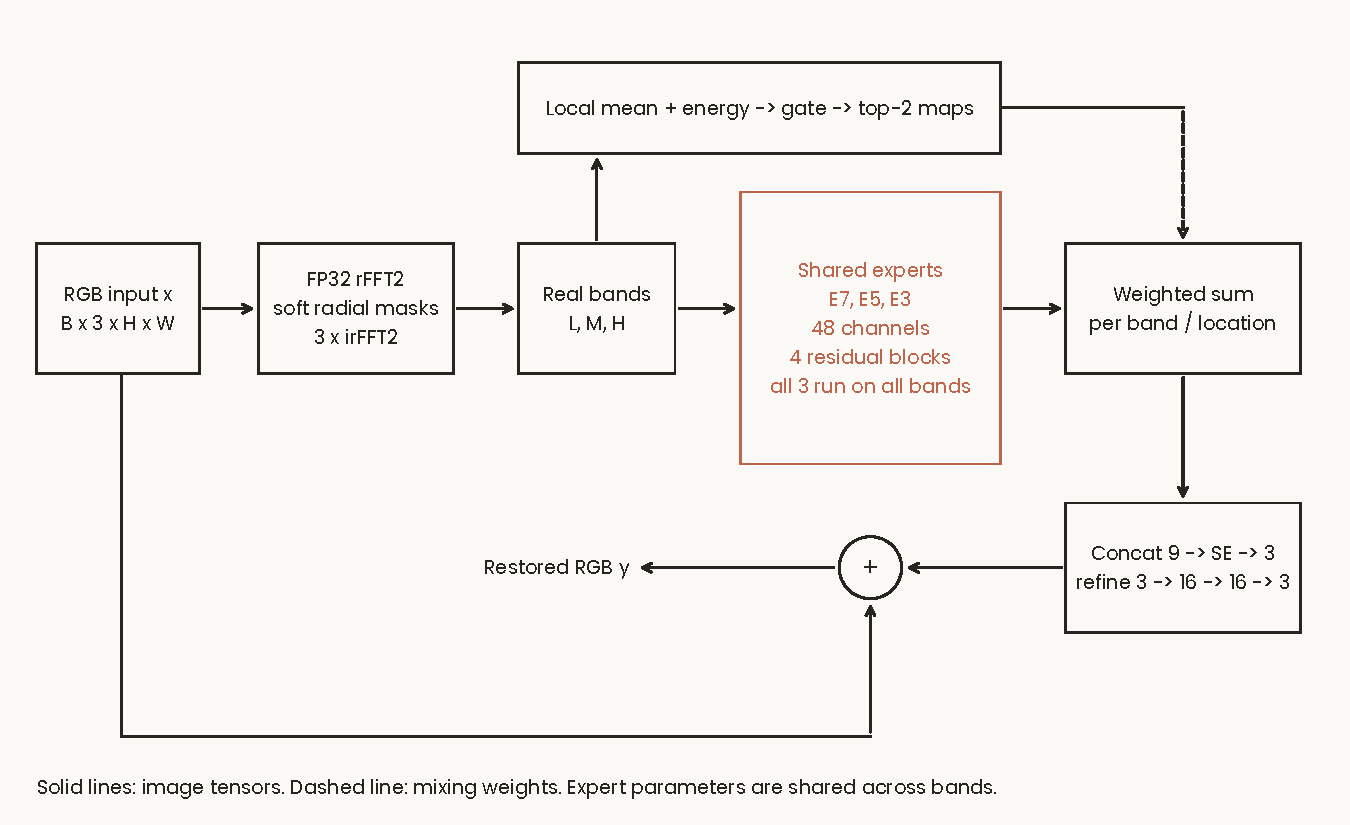
\includegraphics[width=0.95\linewidth]{architecture.pdf}
	\caption{\fcsg{} data flow. The bands share expert parameters.}
	\label{fig:architecture}
\end{figure}

\paragraph{Frequency decomposition.} Let $X$ be the orthonormal real FFT of
$x$ and $r$ the radial frequency in cycles per pixel. A soft low-pass mask
with cutoff $c$ and width $\Delta=0.05$ is
$\mathrm{LP}_c(r)=\tfrac12\big(1+\cos(\pi\,\mathrm{clip}((r-c)/\Delta+\tfrac12,0,1))\big)$.
With $r_1=0.10$ and $r_2=0.25$ the band masks are $M_L=\mathrm{LP}_{r_1}$,
$M_M=\mathrm{LP}_{r_2}-\mathrm{LP}_{r_1}$ and $M_H=1-\mathrm{LP}_{r_2}$, and
$x_b=\mathcal{F}^{-1}(M_b X)$. Three choices matter here. The masks sum to
one, so $x_L+x_M+x_H=x$ exactly. The cutoffs are normalised frequencies, not
FFT bin indices, so a band means the same thing on a $128\times128$ training
crop as on a full image. And each band goes back to the spatial domain before
any learned layer. A convolution over a spectrum has no clear meaning, and
complex inputs make training unstable, so the experts stay plain real-valued
CNNs.

\paragraph{Experts.} Each expert starts with a $2\times2$ pixel unshuffle
\cite{shi2016espcn}, giving 12 channels at half resolution. A $1\times1$
convolution widens these to 48 channels. Four residual blocks follow, each
with two depthwise-separable stages \cite{chollet2017xception} of kernel
$k\in\{7,5,3\}$. A $1\times1$ tail adds back the unshuffled input, and a pixel
shuffle restores full resolution. Separable convolutions at half resolution
are what fit nine expert passes inside the compute budget. We name the
experts by kernel size only, because we have no evidence of what each one
specialises in.

\paragraph{Spatial top-2 gate.} A gate that decided once per image would be
a lookup table, and it would tend to settle on a constant choice. Our gate
pools the mean and the mean of squares of the nine band channels in
$16\times16$ windows. An $18\to24\to9$ network maps these 18 statistics to
one logit per band and expert, and the logits are upsampled to full
resolution. At each pixel the gate keeps the two largest logits per band and
normalises them with a softmax. The third expert gets zero weight. The loss
uses the dense softmax $p_{b,e}$ over all three. The gate has 681 parameters.
The network still computes every expert before mixing.

\paragraph{Fusion and refinement.} The nine band channels go through a
squeeze-and-excitation block \cite{hu2018se}, a $1\times1$ projection to RGB
and three $3\times3$ convolutions ($3\to16\to16\to3$). The output is a
residual added to the input, as in DnCNN.

\section{Training objective}\label{sec:loss}

\begin{equation}
	\mathcal{L}=\mathcal{L}_\text{char}+0.05\,\mathcal{L}_\text{freq}+\lambda_\text{ent}(t)\,\mathcal{L}_\text{ent}.
\end{equation}
The Charbonnier loss \cite{charbonnier1994} is
$\mathcal{L}_\text{char}=\operatorname{mean}\sqrt{(\hat f-f)^2+\varepsilon^2}$
with $\varepsilon=10^{-3}$. $\mathcal{L}_\text{freq}$ is the mean absolute FFT
of the error, which weights all frequencies equally.
$\mathcal{L}_\text{ent}=\sum_b\operatorname{mean}\sum_e p_{b,e}\log p_{b,e}$
is the negative routing entropy. Minimising it keeps all experts in use early
on. Its coefficient decays linearly from 0.01 to 0, which leaves the gate
free to commit by the end. The baselines use the same loss without the
entropy term.

\section{Size and compute}\label{sec:size}

\fcsg{} has 97,088 parameters. The $7\times7$, $5\times5$ and $3\times3$
experts hold 39,228, 30,012 and 23,868. The gate has 681, fusion 96 and
refinement 3,203. We count each multiply-accumulate as two FLOPs and add an
estimate for the FFTs. A $256\times256$ pass then costs 4.66 GMACs, or 9.39
GFLOPs, inside the limit. Section~\ref{sec:cost} shows that this count
predicted running time badly.
